% Diese Zeile bitte -nicht- aendern.
\documentclass[course=asp]{aspdoc}

%newly added packages
\usepackage{microtype}
\usepackage{graphicx}
\usepackage{caption}
\usepackage{wrapfig}
\usepackage{enumitem}
\usepackage{amssymb}
\usepackage{amsthm}
\usepackage{listings}

\usepackage{amsmath}	%eins von beidem?
\usepackage{mathtools}

\usepackage{index}

%%%%%%%%%%%%%%%%%%%%%%%%%%%%%%%%%
%% TODO: Ersetzen Sie in den folgenden Zeilen die entsprechenden -Texte-
%% mit den richtigen Werten.
\newcommand{\theGroup}{132} % Beispiel: 42
\newcommand{\theNumber}{A214} % Beispiel: A123
\author{Mohammed Attia \and Thomas Torggler \and Patrick Zimmermann}
\date{Wintersemester 2020/21} % Beispiel: Wintersemester 2019/20
%%%%%%%%%%%%%%%%%%%%%%%%%%%%%%%%%

% Diese Zeile bitte -nicht- aendern.
\title{Gruppe \theGroup{} -- Abgabe zu Aufgabe \theNumber}

\begin{document}
\maketitle

\newpage
\section{Einleitung} \label{Einleitung}

Raumf\"ullende Kurven bilden eine Br\"ucke zwischen Kunst und mathematischer Geometrie. In der Mathematik werden sie gemeinhin benutzt um ein $n$-dimensionales Problem in ein Eindimensionales zu konvertieren. Eine solche Kurve beschreibt grunds\"atzlich einen linearen Pfad durch $n$-dimensionale R\"aume. Giuseppe Peano war der Erste, der eine solche Kurve 1890 definierte.

Um einen n-dimensionalen Raum in die Dimension n-1 zu konvertieren, l\"asst sich eine stetig, surjektive Funktion $f(x)$ erstellen, so dass gilt: $\forall x \in \mathbb{R}^{n-1} \quad \exists y \in \mathbb{R}^n$. F\"ur einen Beweis der Stetigkeit einer Peano-Kurve siehe~\cite{stetigkeitsBeweis}, f\"ur einen Beweis der Surjektivit\"at solcher Funktionen und tiefere mathematische Definitionen sei auf ~\cite{surjektivBeweis} verwiesen. Hier wollen wir uns auf die sogenannten Peano-Kurven beschr\"anken. F\"ur eine solche Kurve definieren wir ein Intervall $I = [0;1]$, sowie  $f: I \rightarrow I^2 $. Dann ist die Peano-Kurve: $\lim\limits_{n \to \infty}f_n(x)$, mit $n \in \mathbb{N}$. Sie entspricht also dem Grenzwert einer Folge von Funktionen $f(x)$ und l\"asst sich mit der Bedingung, dass sich die Kurve nicht \"uberschneiden darf, folgenderma\ss en konstruieren:

Man unterteile eine Fl\"ache in 9 Quadrate. Jedes dieser Quadrate soll nun von einer Kurve in Form eines 'S' durchlaufen werden.
In einem Iterationsschritt l\"asst sich eines der 9 Quadrate in weitere 9 Quadrate Unterteilen, die wiederum auf dieselbe Art verbunden werden, wie in Abbildung \ref{Abb:Peano} gezeigt.

\begin{figure} [ht] %vorher, eigentlich bild unter text
\centering
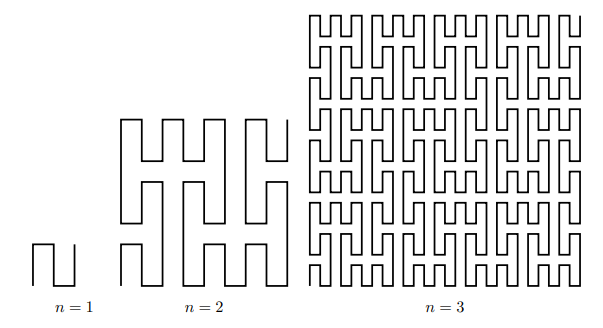
\includegraphics[scale=0.9]{PeanoBsp.png}
\caption{Peano-Kurve mit $n = \{1, 2, 3\}$, ~\cite{aufgabenstellung}}\label{Abb:Peano}
\end{figure}

In Realit\"at sind gesammelte Daten meistens nicht linear, nicht station\"ar und mehrdimensional. Beispiele f\"ur solche Daten sind Matrizen, Bilder, Tabellen und Rechengitter, die sich aus der Diskretisierung von partiellen Differentialgleichungen ergeben. Dateioperationen wie Matrixmultiplikationen, Lade- und Speicheroperationen sowie das Aktualisieren und Partitionieren von Datens\"atzen k\"onnen vereinfacht werden, wenn eine effiziente Methode zum Durchsuchen der Daten gew\"ahlt wird. Die Verwendung dieser komplexen Daten kann zeitlich sehr teuer sein und erh\"ohen die Speicherverwendung exponentiell. Deshalb brauchen wir Kompressions-Algorithmen um unsere Programme optimieren zu k\"onnen. In solchen F\"allen bietet sich die Nutzung der Peano-Kurve oder anderer raumf\"ullenden Kurven an. Eine Transformation eines n-dimensionalen Raumes in die Dimension n-1, f\"uhrt zu einer wesentlichen Komprimierung der Informationen und beh\"alt einen Teil der r\"aumlichen Daten bei. Eine m\"ogliche Anwendung dieses Konzepts ist das Feld des Image Processings bei dem Raumf\"ullende Kurven f\"ur Bild- und Farbkompressionen verwendet werden~\cite{imageProcessing}.

Der Nachteil der vorgeschlagenen Struktur liegt in ihrer relativen Komplexit\"at. Beipielsweise ist in unserer Implementierung bei Grad $n > 9$ die Speicherallokation nicht mehr m\"oglich, wie sp\"ater im Kapitel \ref{Technische Limitationen} erl\"autert wird.

Im Folgenden definieren wir $n \in \mathbb{N}$ als Grad der Kurve.
Wir beschreiben nun unseren Ansatz, einen iterativen Algorithmus mit dem Grad $n$ als Eingabe zu finden, um die eben beschriebene Peano-Kurve darzustellen. Die hierbei generierten Punkte werden in ihrer Reihenfolge ausgegeben. Anders als in der beschriebenen mathematischen Definition werden wir jedoch nicht nur nach $[0;1]$, sondern nach $\mathbb{N}$ abbilden.
Die Korrektheit des hier gew\"ahlten Ansatzes wird gezeigt, in C und in Assembler implementiert und hinsichtlich ihrer Performanz analysiert. Dabei ist zu erkennen, dass eine rekursive Implementierung wahrscheinlich bessere Ergebnisse erziehlt h\"atte und eine Optimierung mit SIMD-Instruktionen die Performanz nur bedingt erh\"oht.

\section{L\"osungsansatz} \label{L\"osungsansatz}

\subsection{Algorithmus} \label{Algorithmus}

Der Aufbau der Peano-Kurve erm\"oglicht es, die Kurve des aktuellen Grades mit einer Variation der originalen Kurve des vorherigen Grades und deren Permutationen zu zeichnen. Wie in Abbildung \ref{Abb:Peano L\"osungsidee} gezeigt gibt es ingesamt drei Permutationen der Kurve:

\begin{itemize}
    \item Die Invertierung, bei der jeder Schritt auf seinen entsprechenden Komplement abgebildet wird.
    \item Die Spiegelung, bei der nur die vertikalen Schritte auf ihren Komplement abgebildet werden.
    \item Die gespiegelte Invertierung, bei der die vorherigen Permuationen kombiniert werden.
\end{itemize}

Diese Observation war der Grundstein des hier beschriebenen iterativen Algorithmus. Anfangs wird dabei die Startkurve hartcodiert in einem Integerarray mit Werten im Interval $[0;3]$ abgespeichert wobei jede Zahl eine Richtungen repr\"asentiert: 0 f\"ur Oben, 1 f\"ur Rechts, 2 f\"ur Unten und 3 f\"ur Links. Die orignale Kurve des ersten Grades und und deren Invertierung sehen wie folgt aus: $\{0, 0, 1, 2, 2, 1, 0, 0\}$ bzw. $\{2, 2, 3, 0, 0, 3, 2, 2\}$. 
Falls $n > 1$ ist, wird startend vom Grad 2 aufsteigend \"uber alle Grade $m \leq n$ iteriert. Bei jeder Iteration wird abwechselnd ein Verbindungschritt entsprechend eines Schritts entlang der Kurve $n = 1$ hartcodiert in den Array geschrieben und danach die entsprechende Permutation der Kurve des vorherigen Grades $m - 1$ berechnet und eingef\"ugt. Dieser Vorgang wird f\"ur die acht fehlenden Teilkurven des aktuellen Grades $m$ ausgef\"uhrt, bis die vollst\"andige Kurve entsteht.

\begin{figure}[ht]
\centering
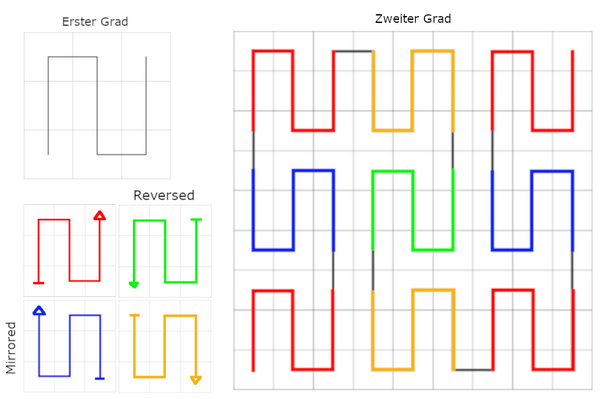
\includegraphics[scale=0.3]{PeanoFarbcodiert.png}
\caption{Peano-Kurve mit $n = 1$, $n = 2$}\label{Abb:Peano L\"osungsidee}
\captionsetup[figure]{font=small,labelfont=small}
\end{figure}

Nachdem \"uber alle Grade iteriert wurde l\"auft der Algorithmus den vollst\"andigen Richtungsarray ab, ver\"andert dabei bei jedem Schritt je nach Richtungsangabe entweder die X oder Y-Koordinate und speichert diese dann in die Ausgabeliste der Peano-Methode.

\subsection{Umgesetzte Optimierungen} \label{Umgesetzte Optimierungen}

Im urspr\"unglichen Entwurf des Algorithmus wurden die drei Permutationen vor jeder Iteration einmal berechnet und als einzelne Arrays abgespeichert um sie danach, wenn sie ben\"otigt werden, nur mehr an die jeweiligen Stellen des Richtungsarrays zu kopieren. Da dadurch jedoch ein erh\"ohter Speicheraufwand entsteht, haben wir uns daf\"ur entschieden jede Permutation immer neu zu berechnen, wenn sie gebraucht wird und diese direkt in den Array zu speichern. Dies schien f\"ur uns ein sinnvoller Optimierungsansatz zu sein, da jede Permutation wie in Abbildung \ref{Abb:Peano L\"osungsidee} zu sehen maximal zweimal vorkommt. Allein die Originalkurve wird dreimal ben\"otigt und auf diese kann immer sehr schnell zugegriffen werden, indem man auf die Werte an den Adressen von $0$ bis $9^{(m - 1)} - 2$ im Richtungsarray zugreift. 

%SIMD
Bei der Assemblerimplementierung beschr\"anken wir uns auf Instruktionen der x86-64-Architektur bis einschlie\ss lich der SSE4.2-Erweiterung~\cite{intel2020man}. Hier haben wir die Funktionen, die die invertierte Permutation erstellt, sowie die Funktion, die die Orginalkurve an die ben\"otigte Stelle des Arrays schreibt, mit SIMD-Befehlen optimiert. 

% Ein calleesaved register weniger verwendet

\subsection{Alternativer L\"osungsansatz} \label{Alternativer L\"osungsansatz}

Abgesehen von den eben beschriebenen Optimierungen wurde bewusst weitgehend auf die Nutzung von SIMD-Befehlen verzichtet, der einzige noch gewinnbringende Anwendungspunkt w\"are die parallele Umrechnung der Richtungen zu den Koordinaten. Die Richtungsberechnung l\"asst sich im Rahmen dieser Arbeit auch nicht mehr gewinnbringend mit SIMD optimieren, da die Funktionen, die weitere Permutationen generieren, in jedem Berechnungsschritt eine Fallunterscheidung besitzten, weshalb hier SIMD nicht zu erhebichen Performanzgewinnen f\"uhren w\"urde. 

Da wir 64-Bit gro\ss e Koordinatenstellen benutzen, k\"onnten wir generell maximal zwei Koordinaten gleichzeitig verrechnen. Da die Koordinatenberechnung allerdings aufeinander aufbaut, wurde sie hier nicht mit SIMD optimiert. Hinzu kommt, dass die Kurve nach zwei Schritten die Richtung \"andert und man nicht mehr dieselbe Berechnung parallel ausf\"uhren kann.

Dennoch w\"urde sich der Algorithmus in einem alternativen L\"osungsansatz zus\"atzlich noch mit Hilfe von SIMD-Instruktionen weiter optimieren lassen.  

Alternativ haben wir gegen Ende der Bearbeitungszeit eine M\"oglichkeit gefunden den Richtungsarray auszulassen und die gesamte Koordinatenberechnung direkt durchzuf\"uhren. Dies w\"urde nat\"urlich sehr viel Rechenaufwand einsparen und damit ingesamt bessere Performanzergebnisse erzielen.

\section{Korrektheit} \label{Korrektheit} % oder Genauigkeit

Die Genauigkeit unseres Algorithmus ist abh\"angig von dem Grad $n$, der die Anzahl an Iterationen bestimmt, wie in Abbildung \ref{Abb:Peano} beschrieben. Das geht auch aus der beschriebenen mathematischen Definition hervor, da die Peano-Kurve an sich ein Grenzwert ist. Somit wird der Algorithmus pr\"aziser, je gr\"o\ss er der Grad der Kurve ist, da die Punkte auf der Kurve sich ebenfalls einem Grenzwert ann\"ahern. Ansonsten ist die Kurve wie oben beschrieben, definiert, weshalb nun die Korrektheit unseres Algorithmus entscheidend ist.
Grunds\"atzlich l\"asst sich die Korrektheit einer Kurve, besonders bei der von uns behandelten, nachweisen, indem man ihre graphischen Darstellungen vergleicht. Da das theoretisch aber nicht m\"oglich ist, folgt auch eine Implementierung in Assembler und in C, die wir auch hinsichtlich ihrer Performanz analysieren wollen.
Dennoch soll der bereits beschriebene Ansatz auf Korrektheit gepr\"uft werden.


Da die eigentliche Koordinatenberechnung abh\"angig von der zuvor ermittelten Richtung ist, ist der folgende Beweis prim\"ar auf die Berechnung der Richtungen ausgerichtet.
Die Koordinatenberechnung findet anschlie\ss end und basierend auf den bisherigen Ergebnissen statt, indem ab\"angig von der Richtung jeweils die X- und die Y-Koordinate eines Z\"ahlers inkrementiert bzw. dekrementiert und abgespeichert wird.

\subsection{Beweis der Permutationen durch Induktion} \label{Beweis der Permutationen durch Induktion}
Nachdem die Kurve immer wieder die gleichen, teilweise elementaren, Bestandteile verwendet, m\"ussen diese und deren Permutationen richtig berechnet werden. Im Speziellen sind das die Kurven mit $n = 1$ und $n = 2$. Aus diesen l\"asst sich induktiv die Korrektheit beweisen, da wir, wie im vorherigen Kapitel \ref{Algorithmus} beschrieben, zum Berechnen einer Kurve $n$-ten Grades nur die Kurve des Grads $n - 1$ sowie die gespiegelte und invertierte Version dieser Kurve benutzen.

\subsubsection{Induktionsbasis} \label{Induktionsbasis}
Beginnen wir mit $n = 1$. Hier ist die Kurve vordefiniert, dementsprechend gibt es nichts zu zeigen. Da auf diesem Muster alle anderen Kurven mit $n > 1$ basieren, ist sie in unserem Algorithmus ebenfalls als Basis vorgegeben.
Des Weiteren ist die Definition der Kurve mit $n = 2$ f\"ur die Berechnung aller weiteren Kurven n\"otig, da man anhand dieser Kurve alle notwendigen Bedingungen der Konstruktion weiterer Kurven ableiten kann. Deshalb nehmen wir sie also auch als definiert an \ref{Abb:Peano}. Diese Bedingungen sollen im folgenden ebenfalls gepr\"uft werden.

\subsubsection{Induktionsannahme} \label{Induktionsannahme}
Da die Funktion wie vorher definiert surjektiv und stetig ist, gilt:

\begin{center}
$\forall n > 1 \in \mathbb{N}$ und $\forall y \in \mathbb{R}^n$ gilt: $\exists x \in [0,1]$ so, dass $f(x)= y$
\end{center}

Dadurch lassen sich Kurven mit h\"oherem Grad konstruieren. Es sei nun $n > 1$ und $n$ beliebig gew\"ahlt.

\subsubsection{Induktionsschritt} \label{Induktionsschritt}
Betrachten wir nun Kurven $n$-ten Grades. Hierzu m\"ussen wir die Permutationen der vorhergehenden Kurve untersuchen, die wir zur Konstruktion der Kurve mit Grad $n$ ben\"otigen.
Da diese Permutationen stets auf \"ahnliche Art konstruiert werden, n\"amlich durch Addition von 2 zu der gespeicherten Richtung mit anschlie\ss endem \textit{modulo} 4, um die Richtung wieder in den g\"ultigen Bereich abzubilden. Dadurch ist gewehrleistet, dass durch Mehrfachanwendung einer Funktion, die eine solche Permutation generiert, immer nur die Orginale Kurve oder die gew\"unschte Permutation entstehen kann. Dies wird durch den Wertebereich von $[0;3]$ und \textit{modulo} 4 erreicht, da so die geraden Werte auf den jeweils anderen geraden Wert abgebildet werden, f\"ur die ungerade Zahlen analog. Dieser Umstand wird bei dem Erstellen der Permutationen ausgenutzt.
Da die Funktionen, die die Permutationen erzeugen, auf die gesamte Kurve des Grades $n = n - 1$ angewand wird, ist sichergestellt, dass die Permutationen keine anderweitigen Fehler in der Richtungsberechnung besitzten. Ergebnis ist in Abbildung \ref{Abb:Peano L\"osungsidee} dargestellt.

\textbf{Die Permutationen: }% - Reverse in Implementierung
Die invertierte Permutation ist im Kern nichts anderes als die normale Peano-Kurve mit anderer Reihenfolge der Koordinatenberechnung, im Speziellen von $p_1=(1,1)$ nach $p_2 = (0,0)$. Dies hat zur Folge, dass sich au\ss er der invertierten Reihenfolge der Punkte an der grundlegenden Kurve nichts \"andert. Somit ist die invertierte Permutation induktiv eben so korrekt wie die zugrundeliegende Kurve niedrigeren Grades, siehe auch Abbildung \ref{Abb:Peano L\"osungsidee}, gr\"une Kurve.

%\textbf{Spiegelung:}% - Mirror in Implementierung
Bei der Spiegelung wird die Kurve an der X-Achse gespiegelt. Wir ver\"andern also die vertikale Richtung, behalten jedoch weiterhin die horizontale Richtung bei. Dadurch wird die vorausgehende Kurve notwendigerweise abge\"andert. Diese zus\"atzliche Operation ist elementar und greift auf die gespeicherte Richtung einer Koordinate direkt zu. Somit hat diese Operation nur indirekt auf die Koordinatenberechnung Einfluss, ohne die Kurve anderweitig zu ver\"andern. Siehe auch Abbildung \ref{Abb:Peano L\"osungsidee}, gelbe Kurve. %wirklich elementar

%\textbf{Kombination Beider Permutationen:}
Abschlie\ss end bleibt noch die Kombination aus den vorangehenden Permutationen, die ebenfalls f\"ur die Konstruktion der Kurve notwendig ist. Diese Permutation ist, \"ahnlich zu der vorherigen Permutation, eine Spiegelung an der Y-Achse. Dabei wird die horizontale Richtung gewechselt und die Vertikale beibehalten. Ansonsten verh\"alt es sich analog zur Spiegelung.
Siehe auch hier Abbildung \ref{Abb:Peano L\"osungsidee}, blaue Kurve.

\textbf{Verbinden der Permutationen: }
Die unterschiedlichen Permutationen der Peano-Kurve werden durch eine ebensolche Kurve mit $n = 1$ verbunden. Dadurch bleiben alle Eigenschaften der Kurve erhalten, da wir keine weiteren Punkte in die Kurve einf\"ugen, sondern nur die Art der graphischen Darstellung ver\"andern. Wir f\"ugen also einen weiteren hartcodiertern Schritt zu den bisherigen Richtungen hinzu, um die Koordinaten sp\"ater korrekt zu berechnen. Dies ist zudem Teil der Definition dieser Kurve.  


\subsection{Technische Limitationen} \label{Technische Limitationen} %in C
Bei dem Testen unseres Programms fallen bei Graden von $n > 6$ bestimmte technische Limitationen unser Rechensysteme auf. 

Zum einen haben wir kein Programm gefunden, dass die generierten .svg Dateien von einer Gr\"o\ss e 21,8 Megabyte (Peano-Kurve mit $n = 7$) \"offnen kann. Mit zunehmendem Grad enth\"alt die .svg Datei logischerweise immer mehr Punkte der Kurve, weshalb die Gr\"o\ss e ebenfalls exponentiell zur Basis 9 steigt. Deshalb m\"ochten wir an dieser Stelle auf das Kapitel \ref{Korrektheit} verweisen, um die Kurve auf selbige zu pr\"ufen.  %selbige gross?

Zum anderen ist es nicht m\"oglich, beliebig viel Speicher zu allokieren, da die von uns benutzte \textit{malloc}-Funktion maximal 17.179.869.184 Bytes auf dem Heap unser Testumgebungen allokieren kann und der Heap zus\"atzlich in seiner Gr\"o\ss e auf Seite der Hardware begrenzt ist. Deshalb k\"onnen wir auf unseren Systemen die Funktion mit maximal $n = 9$ ausf\"uhren, da sonst nicht gen\"ugend Speicher allokiert wird. F\"ur $n = 10$ m\"ussten 27.894.275.208 Bytes allokiert werden, wozu wir nicht im Stande sind. 

Um zu ermitteln, wie viel Speicher wir allokieren k\"onnen, haben wir eine For-Schleife folgenden Typs ausgef\"uhrt:

\begin{lstlisting} %Formatieren! 

u_int64_t *v;
for (u_int64_t i = 1; v = (u_int64_t *) malloc(i); i <<= 1)   
{     
    print(i); free(v);
}
\end{lstlisting}

Zus\"atzlich evaluierte ein Test, der \"uberpr\"uft, ob der von \textit{malloc} zur\"uckgegebenen Pointer bei $n > 9$ NULL ist, auf unseren Testplatformen ausnahmslos zu \textit{true}. % also war NUll

Deshalb ist der Wertebereich von $n$ in den Tests im nachfolgenden Kapitel auf $ n \in [1;9]$ limitiert.

Als ein Beispiel der erstellten .svg Datei f\"ur diesen Algortihmus sei auf Abbildung \ref{Abb:Generierte Kurve Grad 4} verwiesen, welche die erstellte Kurve mit $n = 4$ zeigt. F\"ur $n < 4$ werden Bilder erzeugt, die den Kurven in Abbildung \ref{Abb:Peano} entsprechen. F\"ur $n > 4$ ist die Kurve aufgrund der hohen Dichte in diesem Dokument schwer lesbar darstellbar.

\begin{figure}[ht]
\centering
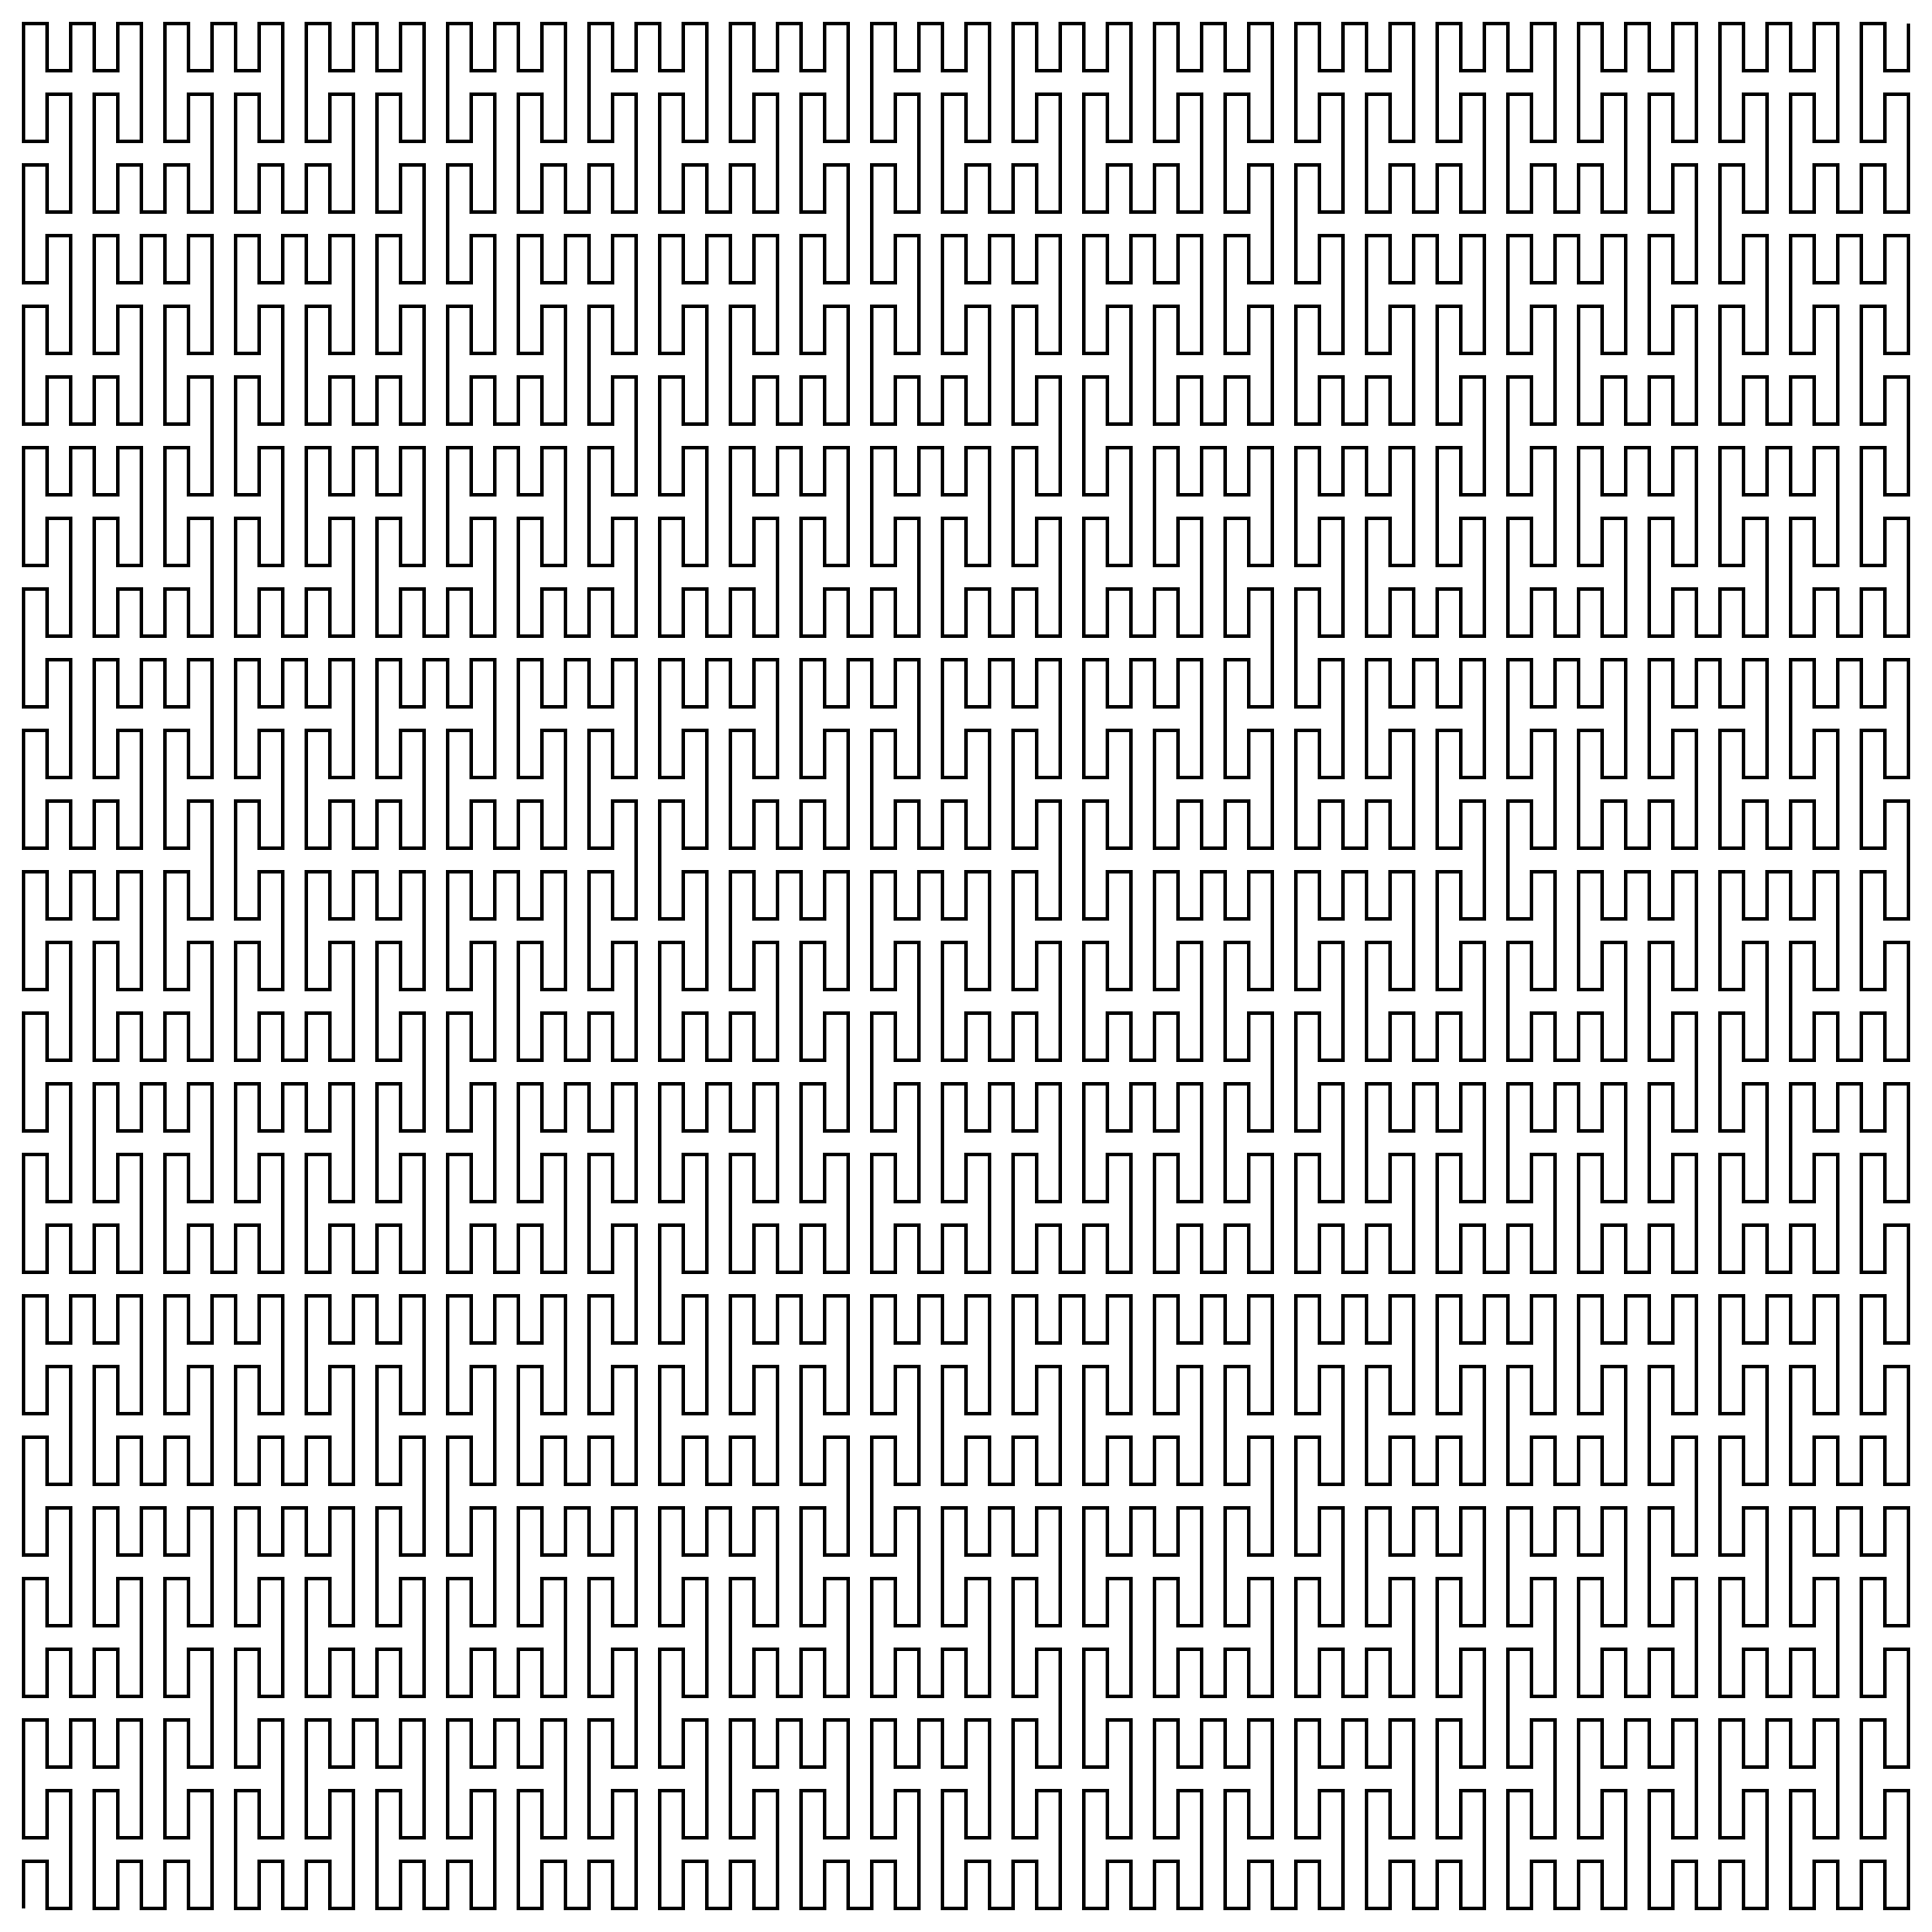
\includegraphics[scale = 0.2]{peanoGrad4.png}
\caption{Generierte Peano-Kurve mit $n = 4$}\label{Abb:Generierte Kurve Grad 4}
\end{figure}

\section{Performanzanalyse} \label{Performanzanalyse}
Bevor der bereits ausgef\"uhrten Algorithmus hinsichtlich seiner Performanz analysiert wird, werden kurz die Algorithmen die verglichen werden, beschrieben.

Als erstes wurde der bereits erl\"auterten Algorithmus aus Kapitel \ref{L\"osungsansatz} in C implementiert. Um die Performanz-Unterschiede zwischen der direkten Berechnung, im Weiteren als In-Place-Variante, und der einmaligen Berechnung und Speicherung der Permutationen, im Folgenden als Out-Of-Place-Variante bezeichnet, zu analysieren erweitern wir die Implementierung um einen entsprechenden Algorithmus, welcher eine abgewandelte Form der In-Place-Variante ist. Der Unterschied besteht darin, dass sobald wir eine Kurve mit $n > 2$ berechnen, speichern wir die schon vorher besprochenen Permutationen der Kurve mit Grad $n - 1$. 

Da wir uns Eingangs auf einen iterativen Ansatz festgelegt haben, ist es zudem interessant zu sehen, inwiefern sich der Unterschied zwischen einem iterativen und einem rekursiven Algorithmus auswirkt. Deshalb wurde auch ein Algorithmus implementiert, der rekursiv die Richtungen berechnet. Aus Zeitgr\"unden k\"onnen wir jedoch die Implementierungen nur in C vergleichen. 

\subsection{Dokumentation}

Die Laufzeittests der verschiedenen Algorithmen wurden auf einem System mit einem Intel Core i7-7700K Prozessor mit einer Taktfrequenz von 4.20GHz, 16 GB Arbeitsspeicher und auf einem Linux Mint 20 64-bit Betriebsssystem mit Linux Kernel 5.4.0-26-generic durchgef\"uhrt. Kompiliert wurde dabei mit GCC 9.3.0 mit Option -03.
Wie bereits im Kapitel \ref{Technische Limitationen} beschrieben, war es nur m\"oglich bis Grad 9 zu testen.
F\"ur jeden Algorithmus wurden f\"ur jeden Grad 20 Durchl\"aufe aufgezeichnet und deren Durchschnitt berechnet. Um das exponentielle Wachstum der Ergebnisse sinnvoll darzustellen werden in der folgendenen Grafik zuerst die Grade 4, 5 und 6 und anschlie\ss end Grad 6 mit 7 und 8 verglichen .

\begin{figure}[ht]
\centering
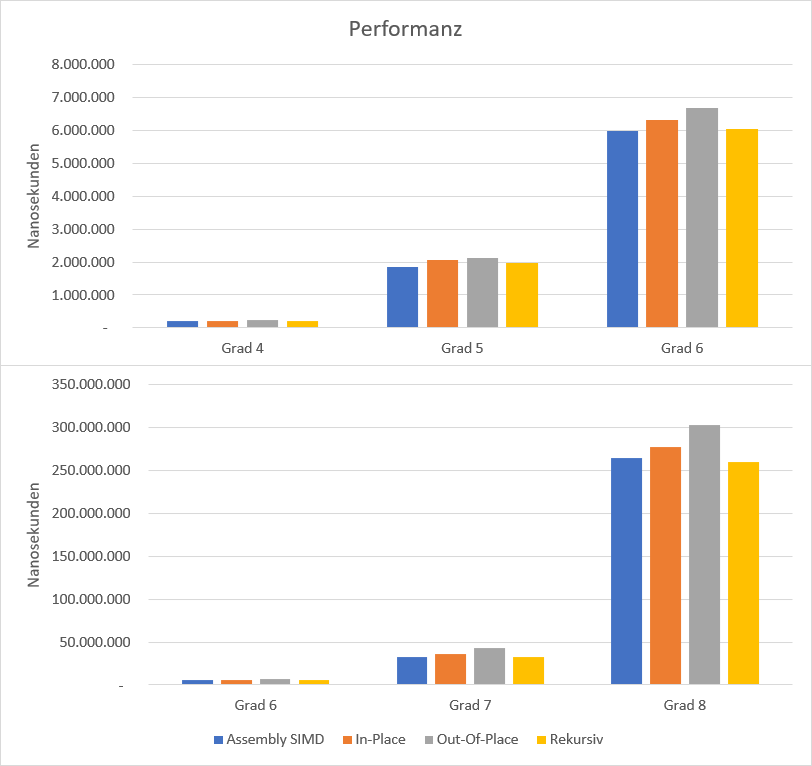
\includegraphics[scale = 0.5]{diagrammeVertikal.png}
\caption{Grafischer Vergleich der Grade 4 bis 8}\label{Abb: Diagramm Performanz}
\captionsetup[figure]{font=small,labelfont=small}
\end{figure}

Zus\"atzlich wird in Abbildung \ref{Abb: Tabelle Performanz} der prozentuelle Zeitunterschied zwischen der SIMD-Optimierten Assemblerimplementierung und den Vergleichsalgorithmen dokumentiert. Hier ist zu erkennen, dass SIMD-Befehle bei den Graden eins bis drei zu deutlichen Zeitverbesserungen von bis zu \"uber 28\% f\"uhren, jedoch bei den Graden f\"unf bis sieben kleinere Zeiteinbusen mit sich bringen. Bei den letzten zwei Graden acht und neun verbessert die Nutzung von SIMD-Befehlen den Algorithmus wieder, jedoch schafft er es nicht die Zeiten des rekursiven Algorithmus zu schlagen.
Damit kann man leider nicht vorhersehen welcher Algorithmus sich f\"ur die Grade $n > 9$ am besten eignen w\"urde oder ob die Verwendung von SIMD-Befehlen bei jedem Grad von Vorteil ist. Es kann jedoch behauptet werden, dass die iterativen Algorithmen in C, In-Place sowie Out-Of-Place, nicht die beste Wahl w\"aren.

\begin{figure}[ht]
\centering
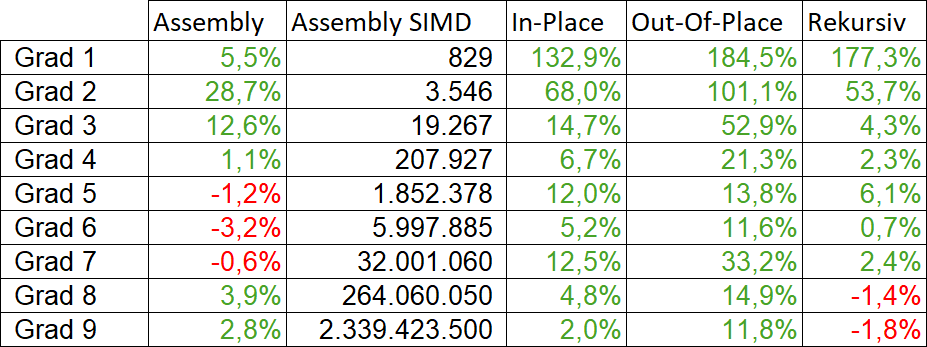
\includegraphics[scale = 0.65]{zeitmessungenProzent.png}
\caption{Prozentueller Performanzvergleich (Zeitangabe in Nanosekunden)}\label{Abb: Tabelle Performanz}
\captionsetup[figure]{font=small,labelfont=small}
\end{figure}

\section{Zusammenfassung und Ausblick} \label{Zusammenfassung und Ausblick}
%Zusammenfassung
Es l\"asst sich also feststellen, dass eine rekursive Implementierung gegen\"uber einem iterativer Ansatz vorzuziehen ist, da in unserer Implementierung der rekursive Algorithmus in den Testf\"allen bis Grad 9 mit Ausnahme $n = 1$ immer besser abgeschnitten hat, vergleiche Abbildung \ref{Abb: Tabelle Performanz}. Zu erwarten war, dass eine manuelle Optimierung des Assemblercodes zu besseren Performanzergebnissen f\"uhrt. Jedoch sind die bisherig implementierten SIMD-Instruktionen bei h\"ohren Graden nicht so performanzsteigernd wie eingangs erhofft wenngleich verst\"andlich, da nicht alle m\"oglichen SIMD-Optimierungen durchgef\"uhrt wurden. Weitere M\"oglichkeiten die Performanz zu erh\"ohen w\"aren Speicheroptimierungen, Multithreading, ein 16-Bit Alignment der SIMD-Instruktionen oder die im Kapitel \ref{Alternativer L\"osungsansatz} beschriebenen Alternativen.

%Ausblick Mo
Ein verbesserter Ansatz des Algorithmus w\"are beispielsweise durch ein Verzicht auf das Richtungsarray zu erreichen. Einen solchen Algorithmus haben wir in C implementiert, dieser verfolgt das selbe Konzept aber arbeitet direkt mit den Koordinaten. Damit l\"asst sich die Speicherverwendung optimieren und die \"uberfl\"ussigen Schritte beim Iterieren \"uber das Array werden eingespart. Wie man auf der Abbildung X sehen kann, hat die neue Variante den Vorteil im Vergleich zur alter Implementierung ..(Analysis of the Figure of the results of the performance of the new Algorithm).

R\"uckblickend ist zu bemerken, dass es wahrscheinlich sinnvoller gewesen w\"are, diesen Ansatz direkt zu verfolgen, da dadurch sehr viel unn\"otige Rechenzeit gespart werden w\"urde.

%Hilbert vs Peano
Betrachtet man die Historie der Raumf\"ullenden Kurven, so f\"allt schnell auf, dass noch weitere Kurven existieren, die vergleichbare Eigenschaften zu der Peano-Kurve aufweisen. Eine solche Kurve w\"are die Hilbert-Kurve, welche den Raum in vier anstatt neun Teile unterteilt. Es bietet sich also an, die hier ausgef\"uhrte Kurve mit beispielsweise der Hilbert-Kurve oder anderen Arten der Peano-Kurve ~\cite{raumKurven}, welche den Raum auf andere Weise durchl\"auft, zu vergleichen.

%Idee am ende, keine Zeit zur Umsetztung, statt inplace direkt Koordinatenberechnung

\newpage
% TODO: Fuegen Sie Ihre Quellen der Datei Ausarbeitung.bib hinzu        !!!!
% Referenzieren Sie diese dann mit \cite{}.
% Beispiel: CR2 ist ein Register der x86-Architektur~\cite{intel2017man}.
\bibliographystyle{plain}
\bibliography{Ausarbeitung}{}

\end{document}
